\section{Architettura}

Approfondiamo l'architettura scelta per Easy-Meal, spiegando le scelte
architetturali e i pattern utilizzati per lo sviluppo dell'applicazione partendo
dalla struttura generale del sistema e passando poi ai dettagli implementativi.

\subsection{Architettura di Deployment}

SWEnergy ha deciso di adottare un'architettura monolitica a tre livelli (\textit{3-tier
architecture}) per implementare Easy-Meal. 
Questa scelta è stata determinata dalla necessità di costruire una 
web application che permetta agli utenti di accedere al sistema da qualsiasi 
dispositivo connesso a Internet. L'architettura a tre livelli
separa la logica di presentazione dalla logica di \textit{business} e dal \textit{database}.
I livelli comunicano tra loro attraverso interfacce ben definite, in particolare:
\begin{itemize}
	\item \textbf{Livello di Presentazione (\textit{Frontend})}: rappresentato da Angular, riceve i dati dall'utente e visualizza i risultati restituiti dal \textit{backend}.
	\item \textbf{Livello di Logica Applicativa (\textit{Backend})}: rappresentato da NestJS. Gestisce la logica di \textit{business}, elabora le richieste provenienti dal frontend e interagisce con il database per recuperare o salvare i dati.
	\item \textbf{Livello di Dati (\textit{Database})}: rappresentato dal \textit{database} PostgreSQL, si occupa della gestione dei dati.
\end{itemize}

Questo approccio ha permesso al team di sviluppo di lavorare in modo parallelo 
sul \textit{frontend} e sul \textit{backend}, riducendo i tempi di sviluppo e 
facilitando il 
testing del sistema. Inoltre, offre la possibilità di scalare ciascuno 
livello separatamente, in modo da garantire prestazioni ottimali e una 
maggiore flessibilità. Infine, è possibile sostituire l'implementazione di 
uno dei livelli senza dover toccare gli altri, garantendo una maggiore 
manutenibilità del sistema.
In particolare lo sviluppo di Easy-Meal è cominciato partendo dal database,
l'elemento su cui abbiamo posto maggiore enfasi, in quanto è il cuore del
sistema. Successivamente sono stati sviluppati il \textit{backend} e il
\textit{frontend}, in modo da garantire una corretta integrazione tra i
diversi livelli dell'applicazione. SWEnergy ha deciso di utilizzare questa
metodologia, perché le funzionalità messe a disposizione da Easy-Meal al livello
della logica di \textit{business} sono principalmente delle semplici operazioni CRUD, che non richiedono
un'interazione complessa tra i diversi livelli dell'applicazione.

\subsection{Pattern Architetturali}

Easy-Meal è stato sviluppato utilizzando due pattern architetturali:
Model-View-Controller e Dependency Injection. Infatti, SWEnergy ha scelto di
adottare Angular e NestJS, due framework che implementano questi pattern in modo
nativo, garantendo una struttura ben definita e una maggiore manutenibilità del
codice.

\subsubsection{Model-View-Controller}

Il pattern architetturale Model-View-Controller (MVC) è stato utilizzato per
suddividere le responsabilità tra i diversi componenti dell'applicazione. In
particolare, il \textit{model} rappresenta i dati dell'applicazione e fornisce i
metodi di accesso e di modifica di tali dati. NestJS è il framework che
implementa il backend nell'applicativo e fornisce le api di accesso ai dati
di modifica tramite i \textit{controller}. Angular, invece, è il framework che
implementa il frontend e fornisce le interfacce grafiche per la gestione delle
interazione con l'utente, ovvero la \textit{view}. I \textit{component} e i
\textit{controller} sono responsabili di gestire le interazioni tra la 
\textit{view} e il \textit{model},
aggiornando i dati in base alle azioni dell'utente. L'aggiornamento della
visualizzazione dei dati è gestito da Angular, che attraverso il \textit{data
binding} permette di mantenere sincronizzati i dati presenti nel \textit{model}
con la \textit{view}.

\subsubsection{Dependency Injection}

Il pattern Dependency Injection (DI) è stato utilizzato per gestire le
dipendenze tra i diversi componenti dell'applicazione. In particolare, Angular
utilizza la DI per iniettare i servizi all'interno dei componenti, permettendo
di scrivere codice più modulare e manutenibile. NestJS, invece, utilizza la DI
per iniettare i servizi all'interno dei controller, permettendo di separare la
logica di business dalla logica di accesso ai dati. Questo approccio consente di
creare componenti indipendenti e riutilizzabili, facilitando la manutenibilità
dell'applicazione. Infine la divisione in moduli rende il codice facilmente
testabile, in quanto è possibile sostituire i servizi con dei \textit{mock} per
testare i componenti in modo isolato.

\subsection{\textit{Frontend}}

Di seguito sono proposti alcuni diagrammi delle classi per il \textit{frontend}
di Easy-Meal. Poiché la struttura del \textit{frontend} è piuttosto vasta, ma
ridondante, nel senso che il pattern \textit{dependency injection} è applicato
allo stesso modo per tutti i componenti, si è deciso di selezionare alcuni
esempi significativi.

\subsubsection{GenericService}

\begin{figure}[H]
	\centering
	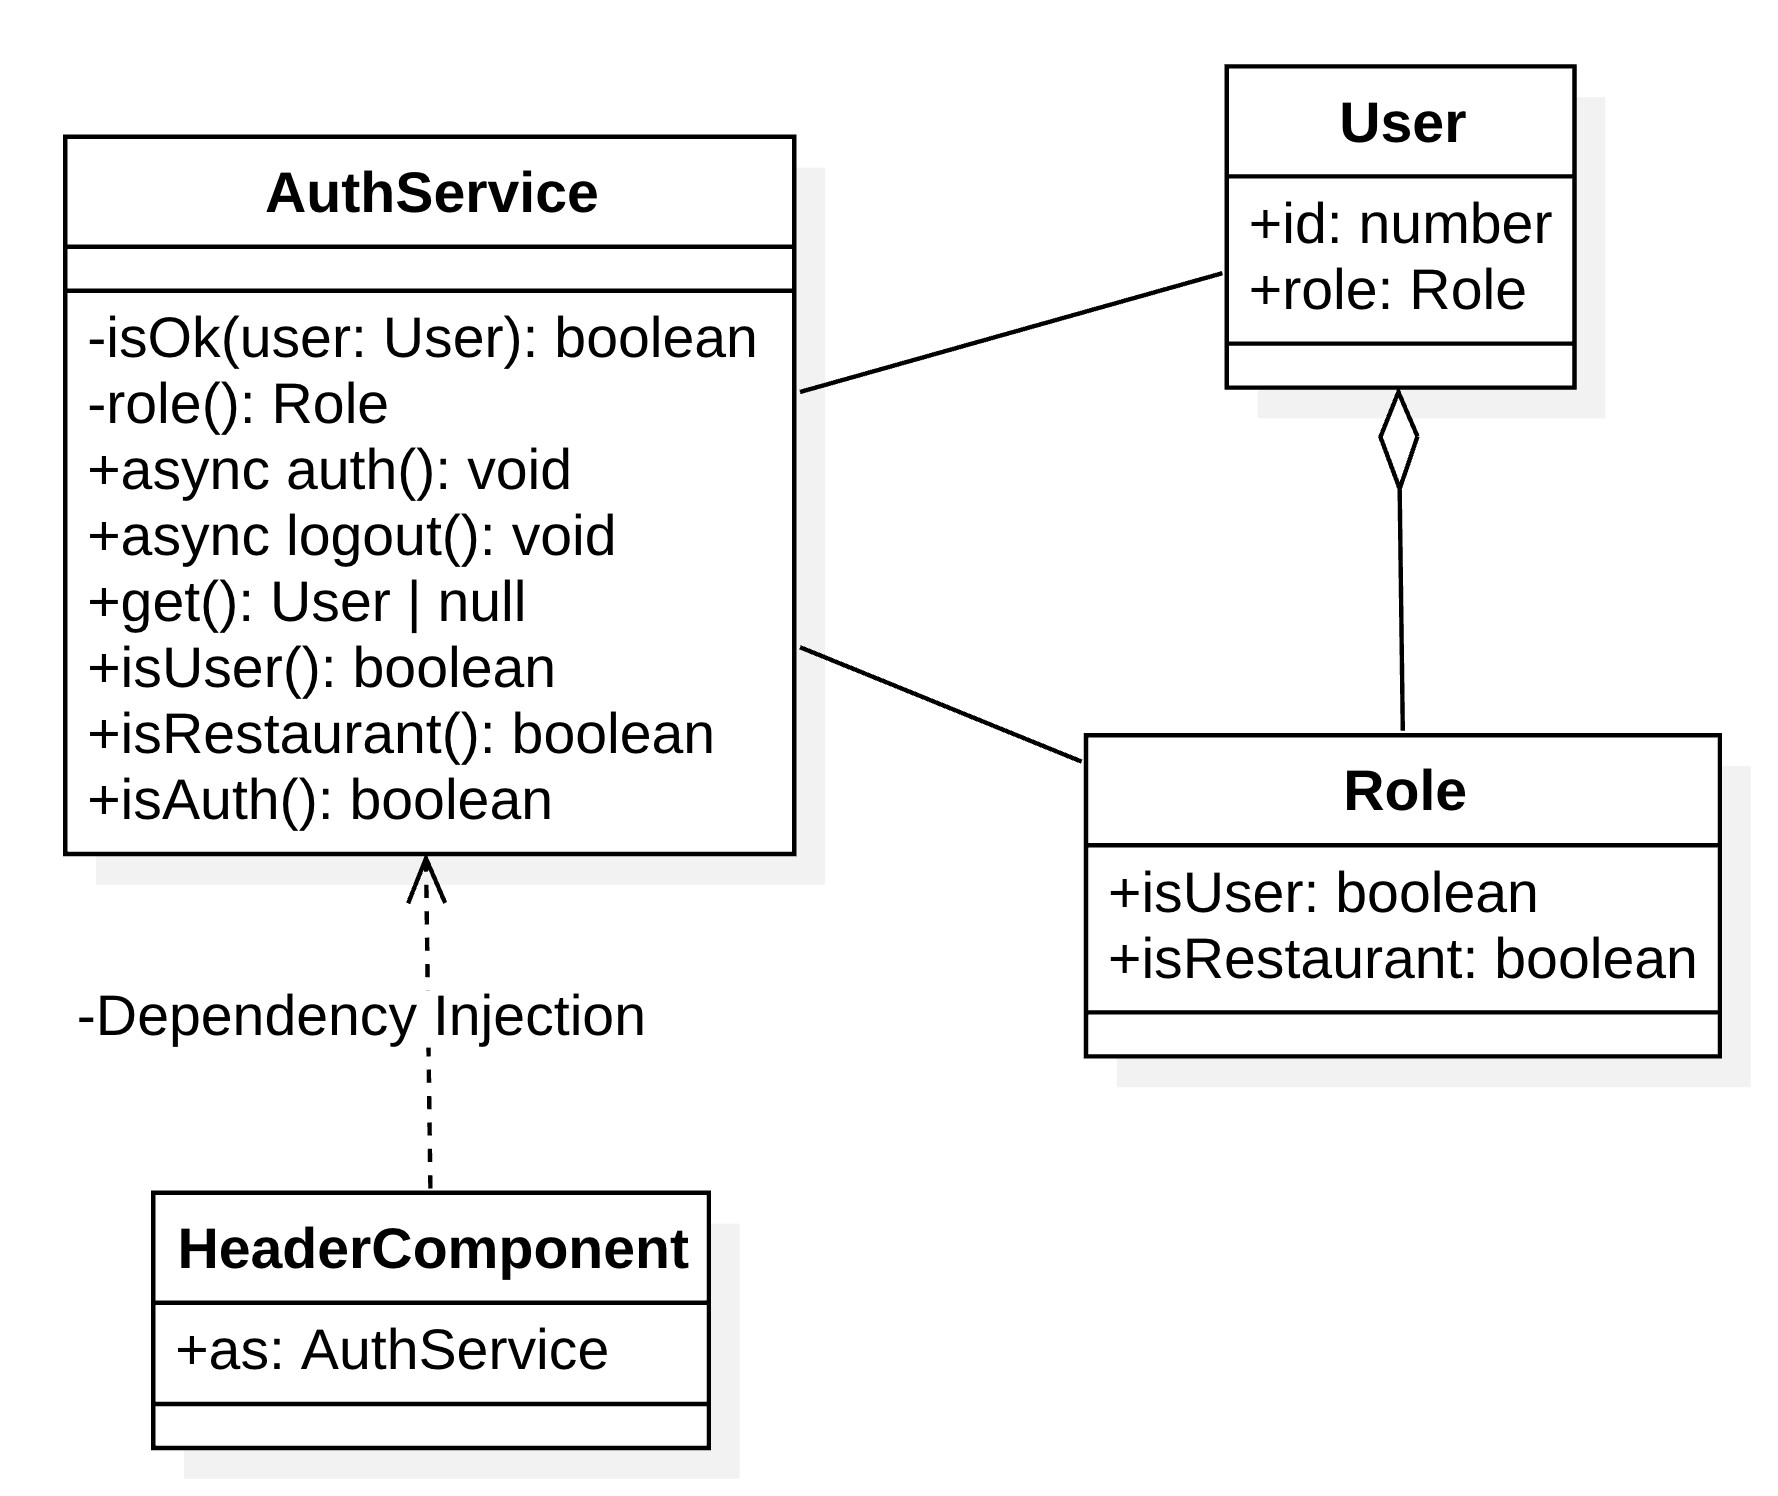
\includegraphics[width=0.5\textwidth]{PB/specifiche-tecniche/auth-service.png}
	\caption{Diagramma delle classi per AuthService}
\end{figure}

In questo caso, viene mostrato come viene iniettato un servizio all'interno di
un componente. Lo \textit{specimen} scelto è il servizio AuthService,
che è responsabile della gestione dell'autenticazione dell'utente. Iniettando
AuthService all'interno del componente HeaderComponent, i metodi pubblici
definiti in AuthService possono essere utilizzati per gestire l'autenticazione
dell'utente. In particolare, HeaderComponent utilizza AuthService per gestire i
link del menu di navigazione in base allo stato di autenticazione e al ruolo 
dell'utente. In questo modo viene favorita la separazione delle responsabilità
e la modularità del codice, rendendo il componente HeaderComponent più
manutenibile e permettendo di riutilizzare AuthService in altri componenti.

\subsubsection{MessageService}

\begin{figure}[H]
	\centering
	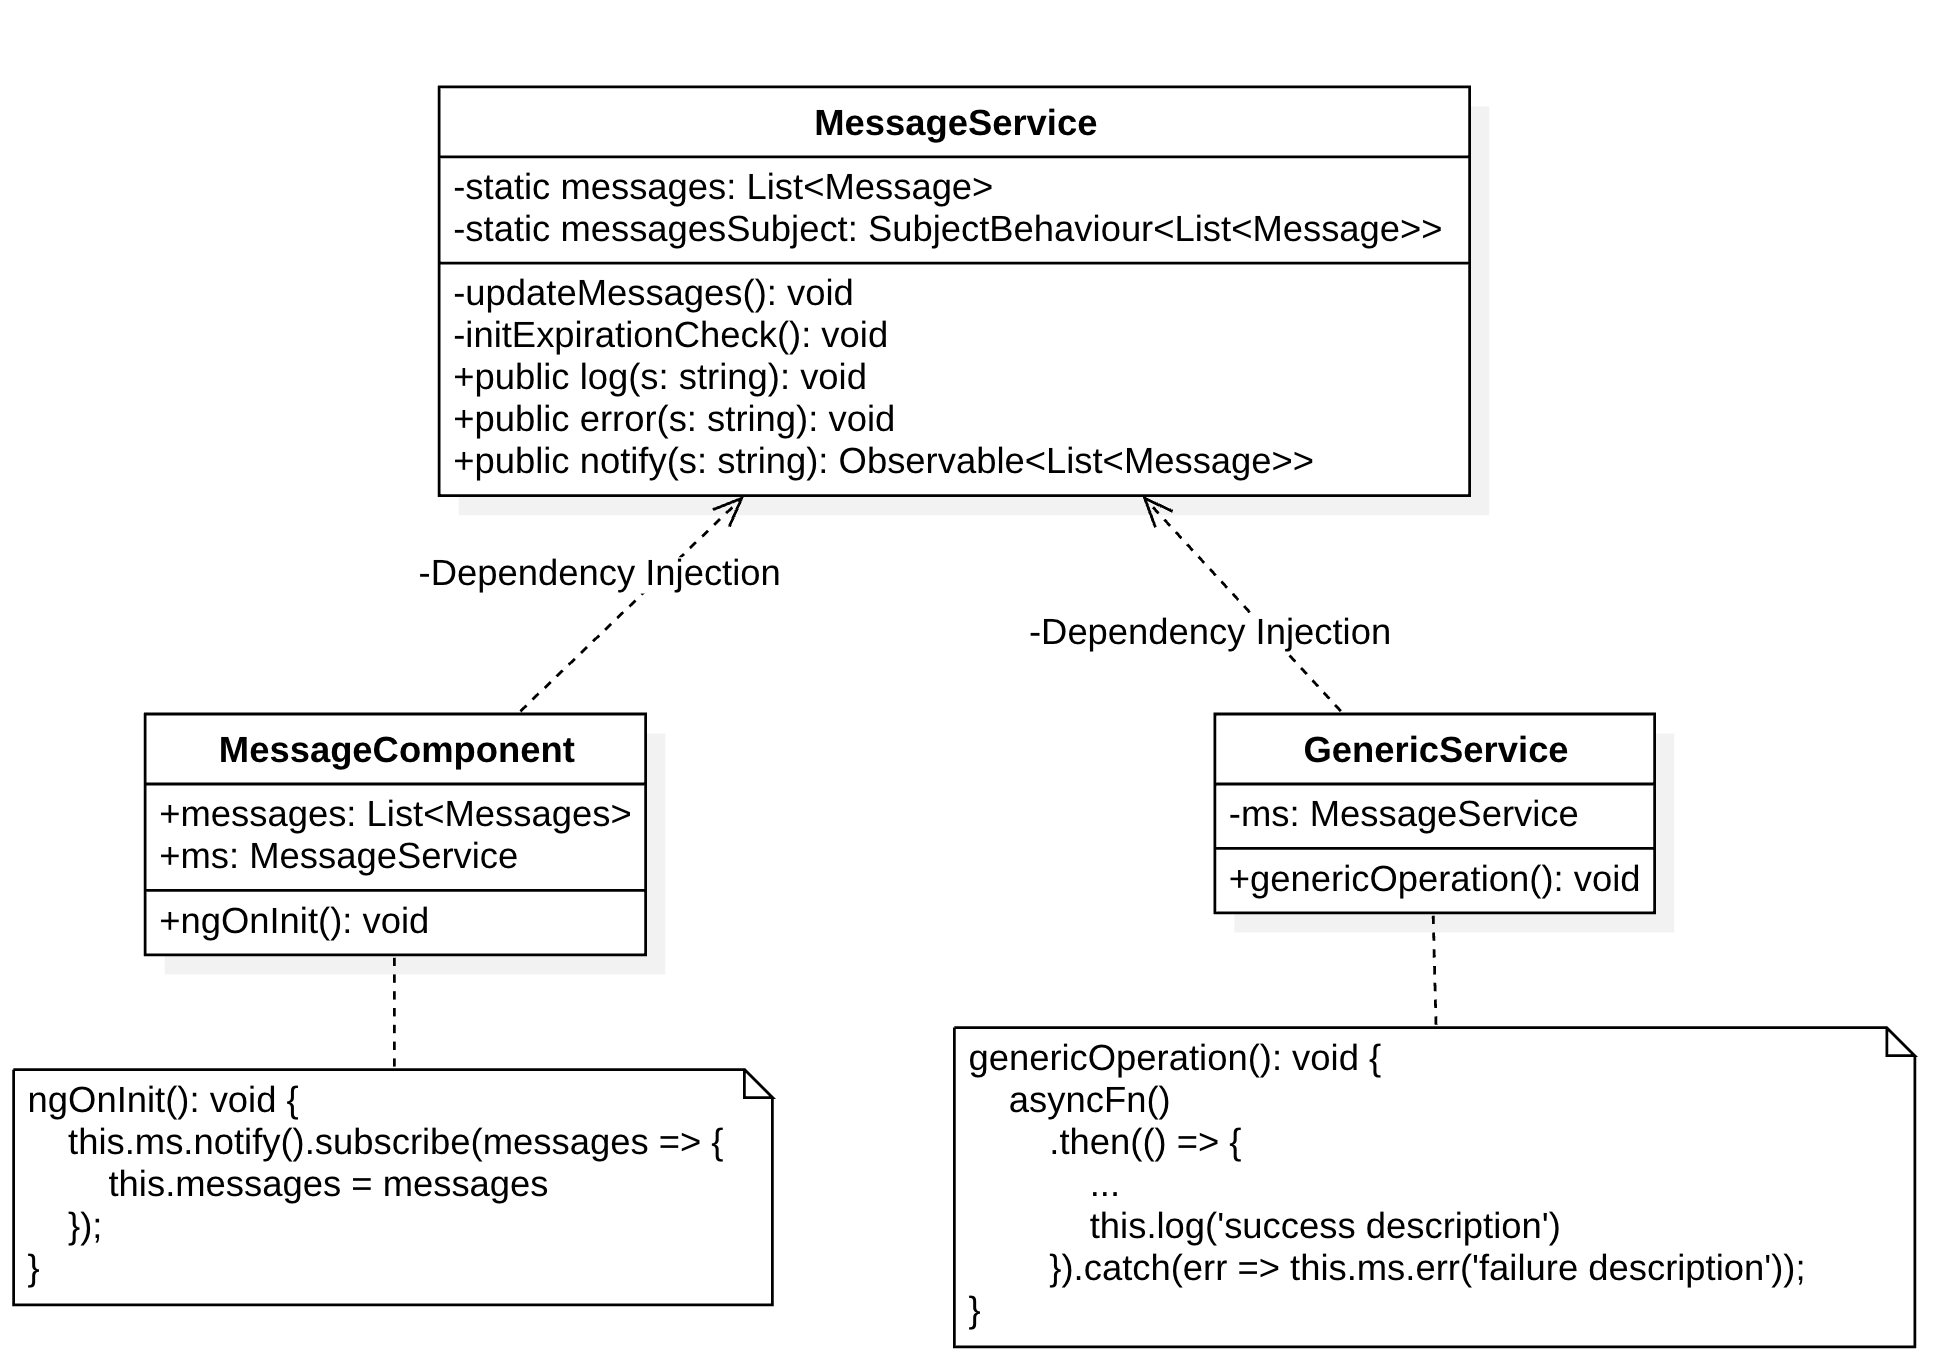
\includegraphics[width=0.8\textwidth]{PB/specifiche-tecniche/message-service.png}
	\caption{Diagramma delle classi per il MessageService}
\end{figure}

La \textit{dependency injection} (DI) in Angular è un \textit{design pattern} che 
consente di fornire dipendenze alle classi in modo automatizzato. In questo 
caso, la classe MessageService viene iniettata sia nella classe 
MessageComponent che nella classe GenericService.
Questo è reso possibile dichiarando MessageService come dipendenza nei 
costruttori delle rispettive classi.
L'annotazione \texttt{@Injectable} viene utilizzata sulla classe MessageService 
per indicare che questa può essere iniettata come dipendenza.\\
MessageService è implementato come singleton in Angular. Un singleton garantisce 
che una sola istanza della classe venga creata e condivisa in tutta 
l'applicazione.
Questo è importante per la gestione centralizzata dello stato e delle operazioni 
comuni, come la gestione dei messaggi.
In Angular, il pattern singleton è implicitamente implementato tramite il 
sistema DI, poiché il servizio è registrato nel \textit{root injector}, 
garantendo una singola istanza.\\
Angular offre un potente meccanismo di \textit{data binding} che consente alla 
vista di aggiornarsi automaticamente quando i dati del modello cambiano.
Nella classe MessageComponent, il metodo \texttt{ngOnInit} utilizza 
l'osservabile restituito da ms.notify() per iscriversi agli aggiornamenti dei 
messaggi.
Quando i messaggi vengono aggiornati nel MessageService, la vista associata a 
MessageComponent si aggiorna automaticamente per riflettere i nuovi dati.
Questo è facilitato dall'utilizzo di Subject o BehaviorSubject in 
MessageService, che emettono nuovi valori quando i messaggi cambiano.\\
In sostanza, in questo modo si utilizza un servizio per condividere dati tra
componenti che non hanno una relazione gerarchica.



\subsection{\textit{Backend}}
Il backend dell'applicazione è stato realizzato utilizzando NestJS, il quale sfrutta diversi pattern creazionali, strutturali ed architetturali.

\subsubsection{Dependency Injection}
Gestisce la creazione delle dipendenze. 
NestJS integra nativamente un sistema di \textit{Dependency Injection} che semplifica l'iniezione delle dipendenze tra i vari componenti dell'applicazione. 
Utilizza il concetto di \textit{provider} per registrare e risolvere le dipendenze.
Un esempio di utilizzo è la registrazione e l'iniezione di servizi nei moduli, generalmente eseguita come nel codice di esempio sottostante.
\begin{lstlisting}
	import { Injectable } from '@nestjs/common';

	@Injectable()
	export class UsersService { // Implementation }
	
	import { Module } from '@nestjs/common';
	import { UsersService } from './users.service';
	
	@Module({
	  providers: [UsersService],
	  exports: [UsersService],
	})
	export class UsersModule {}
\end{lstlisting}
I vantaggi nell'utilizzo della Dependency Injection sono:
\begin{itemize}
	\item \textbf{Separazione delle Preoccupazioni}: migliora la modularità e la manutenibilità del codice.
	\item \textbf{Riusabilità del Codice}: i componenti possono essere riutilizzati in diverse parti dell'applicazione senza dover gestire manualmente le loro dipendenze.
	\item \textbf{Testabilità}: semplifica il testing unitario poiché consente di sostituire facilmente le dipendenze con versioni mock durante i test.
	\item \textbf{Flessibilità e Scalabilità}: consente di sostituire o estendere facilmente le dipendenze senza modificare il codice esistente.
\end{itemize}


\subsubsection{Module Pattern}
Il codice dell'applicazione è suddiviso in moduli, ognuno dei quali incapsula una funzionalità specifica. 
I moduli possono importare altri moduli, rendendo l'applicazione altamente modulare e facilmente manutenibile.
Ogni modulo può contenere \textit{controller}, servizi, \textit{provider} e altre risorse.
I moduli in NestJS sono definiti usando il decoratore "Module", che specifica i componenti che fanno parte del modulo e le loro dipendenze.
\begin{lstlisting}
	import { Module } from '@nestjs/common';
	import { UsersService } from './users.service';
	import { UsersController } from './users.controller';
	
	@Module({
	  providers: [UsersService],
	  controllers: [UsersController],
	})
	export class UsersModule {}
\end{lstlisting}
I vantaggi dell'utilizzo del \textit{Module Pattern} includono:
\begin{itemize}
	\item \textbf{Organizzazione del Codice}: aiuta a mantenere il codice ben organizzato, rendendo più facile trovare e gestire le parti dell'applicazione.
	\item \textbf{Manutenibilità}: ogni modulo può essere sviluppato e manutenuto indipendentemente dagli altri.
	\item \textbf{Riusabilità}: possono essere riutilizzati in altre applicazioni o parti della stessa applicazione.
	\item \textbf{Scalabilità}: facilitando la gestione delle dipendenze e la composizione dei moduli, il Module Pattern supporta la scalabilità dell'applicazione.
\end{itemize}


\subsubsection{Controller-Service Pattern}
NestJS separa la logica di presentazione dalla logica di \textit{business}. \\
I controller sono responsabili di gestire le richieste HTTP, mappando le richieste ai metodi appropriati e restituendo le risposte agli utenti.
Fungono da intermediari tra il \textit{client} (\textit{frontend}) e la logica di \textit{business} dell'applicazione.
Gestiscono la validazione dei parametri in ingresso e la formattazione delle risposte rilasciate.\\
I servizi contengono la logica di \textit{business} dell'applicazione. 
Sono responsabili dell'interazione con il \textit{database}, la gestione dei dati e l'implementazione delle regole di \textit{business}.
Forniscono metodi che possono essere chiamati dai \textit{controller} o da altri servizi.
Contengono operazioni CRUD, manipolazione dei dati e comunicazione con altre parti dell'applicazione.\\
Questo \textit{pattern} promuove una chiara separazione delle responabilità.
\begin{lstlisting}
	import { Controller, Get } from '@nestjs/common';
	import { UsersService } from './users.service';
	
	@Controller('users')
	export class UsersController {
	  constructor(private readonly usersService: UsersService) {}
	
	  @Get()
	  findAll() {
		return this.usersService.findAll();
	  }
	}
\end{lstlisting}
I vantaggi nell'utilizzo del \textit{Controller-Service Pattern} includono:
\begin{itemize}
	\item \textbf{Separazione delle Responsabilità}: separando la logica di presentazione (\textit{controller}) dalla logica di \textit{business (service)}, il codice diventa più modulare e facile da gestire.
	\item \textbf{Manutenibilità}: le modifiche alla logica di \textit{business} non influenzano direttamente la logica di presentazione e viceversa, rendendo il codice più manutenibile.
	\item \textbf{Testabilità}: i servizi possono essere facilmente testati in isolamento senza la necessità di simulare richieste HTTP, migliorando la copertura dei test.
	\item \textbf{Riusabilità}: la logica di \textit{business} incapsulata nei servizi può essere riutilizzata in diverse parti dell'applicazione o in altre applicazioni.
\end{itemize}


\subsubsection{Decorator Pattern}
Il \textit{pattern decorator} è ampiamente utilizzato in NestJS per definire metadati e configurare i componenti dell'applicazione. 
I decoratori in NestJS sono funzioni che possono essere applicate a classi, metodi, proprietà o parametri per arricchirli con comportamenti aggiuntivi o configurazioni specifiche. 
Questo \textit{pattern} permette di aggiungere funzionalità in modo dichiarativo e modulare.
I decoratori più utilizzati nell'applicativo sono:
\begin{itemize}
	\item \textbf{Module}: definisce una classe come modulo NestJS, aggregando \textit{controller, provider}, e altri moduli.
	\item \textbf{Controller}: definisce una classe come \textit{controller} che gestisce le richieste HTTP per un determinato percorso.
	\item \textbf{Provider}: marca una classe come un \textit{provider} (Injectable) che può essere iniettato tramite il sistema di \textit{Dependency Injection} di NestJS.
	\item \textbf{Gestione delle Rotte HTTP}: associa un metodo del controller a una specifica rotta HTTP.
	\item \textbf{Intercettori}: applica uno o più \textit{interceptor} a un metodo specifico.
	\item \textbf{Decoratori per Parametri della Rotta}: estrae parametri dalla rotta e li passa come argomenti al metodo del controller.
	\item \textbf{Decoratori per il Corpo della Richiesta}: estrae il corpo della richiesta e lo passa come argomento al metodo del controller.
\end{itemize}


\subsubsection{Interceptor Pattern}
Gli \textit{interceptor} in NestJS permettono di gestire il comportamento delle richieste e delle risposte in modo centralizzato. 
Possono modificare, trasformare, o loggare i dati prima che vengano inviati al client o al server.
In particolare ne è stato fatto uso per la gestione del caricamento delle immagini relative ai ristoranti ed ai piatti registrati dai ristoratori.
\begin{lstlisting}
	@UseInterceptors(FileFieldsInterceptor([
		{ name: 'logo', maxCount: 1 },
		{ name: 'banner_image', maxCount: 1 },
	  ]))
	  async create(
		@UploadedFiles() files: { logo?: Express.Multer.File[], banner_image?: Express.Multer.File[] }
	  ) {
		// Implementation
	  }
\end{lstlisting}
